\chapter{Análisis de resultados} \label{cap:analisideresultado}

En este capitulo se analizan los distintos resultados obtenidos en nuestros experimentos, detallados en la \autoref{cap:experimentos}, se comparan con los de Bansal \etal~\cite{bansal2018zero} y se explican las diferencias obtenidas.

\section{Resultados cuantitativos} \label{sec:resultadoscuantitativos}

Esta sección desarrolla de forma numérica los resultados obtenidos por los distintos modelos y en las distintas métricas. Desde que se empezó con este trabajo, se publicaron varios artículos sobre ZSD, por lo cual resulta interesante comparar con un trabajo mas actual, y así ilustrar la evolución que obtuvo ZSD en los últimos años.\\\\

\begin{table}[]
	\centering
	\resizebox{12.5cm}{1cm} {
		\begin{tabular}{|l|c|c|c|c|c|}
			\hline
			\multicolumn{1}{|c|}{\textbf{Metrica}} & \textbf{Baseline \cite{bansal2018zero}} & \multicolumn{1}{l|}{\textbf{DSES \cite{bansal2018zero}}} & \textbf{Nuestros con VGG} & \textbf{Nuestros con ResNet} & \multicolumn{1}{l|}{\textbf{Mejor  resultado de \cite{rahman2020zero}}} \\ \hline
			\textbf{100@Recall (Bansal)}           & 22.14                    & 27.19                                                & 26.34                     & 28.91                        & -                                                                      \\ \hline
			\textbf{100@Recall}                    & -                        & -                                                    & 2.72                      & 4.26                         & 12.27                                                                  \\ \hline
			\textbf{mAP@0.5}                       & 0.32                     & 0.54                                                 & 0.19                     & 0.23                        & 5.05                                                                   \\ \hline
			\textbf{mAP@[.5, .95]}                 & -                        & -                                                    & 0.17                     & 0.21                        & -                                                                      \\ \hline
		\end{tabular}
	}
	\caption{Resutados obtenidos por Bansal \etal~\cite{bansal2018zero}, nosotros y Rahman \etal~\cite{padilla2020survey}.}
	\label{tab:resultadosZSD}
\end{table}

La \autoref{tab:resultadosZSD}, muestra los valores de las métricas \textit{100@Recall}, en la versión desarrollada por Bansal  \etal~\cite{bansal2018zero} y la de Padilla \etal~\cite{padilla2020survey}, también se muestran los resultados para \textit{mAP@0.5} y \textit{ mAP[.5, .95]}. Se analizan 2 modelos propuestos por nosotros utilizando \textit{VGG16} y \textit{Inception ResNet V2} y el mejor resultado presentado por el trabajo de Rahman \etal~\cite{rahman2020zero}. Se eligió este documento ya que aborda de una manera similar a la nuestra el problema de ZSD, aunque presenta algunas mejoras y un modelo mas complejo.\\

El mejor resultado de Bansal el cual denomina \textit{Densely Sampled Embedding Space (DSES)} consiste en aumentar el procedimiento de entrenamiento con datos adicionales de fuentes externas que contienen casillas que pertenecen a clases distintas a las clases invisibles. Obtiene 27.19 puntos, el cual nuestro baseline iguala e incluso supera con 26.34 con \textbf{VGG} y 28.91 usando \textbf{ResNet}. El motivo de esto, se debe a que en un principio se calculaba 100@Recall, con una implementación distinta de Bansal. Al no poder igualar sus resultados, se experimento mucho con los distintos parámetros de cada etapa. Luego al calcular con una implementación como define Bansal, esta experimentación resulta en una pequeña mejora en el baseline.

En cuanto mAP, Bansal no aporta mucha información solo reporta los valores para COCO. La implementación es desconocida, por lo cual asumimos que lo reportado es mAP@0.5. De inmediato se puede observar que los valores son muy bajos 0.54. Aunque nosotros obtuvimos resultados aun mas bajos, con un máximo de 0.23 puntos. La justificación de esta diferencia es, que Bansal solo tiene en cuenta aquellos cuadros verdaderos que tienen un IOU $> 0.5$ con alguna propuesta. Pero nosotros utilizamos todos los cuadros verdaderos, independientemente si se detectaron o no. 
	
Si aislamos nuestros resultados, sabiendo que es solo un baseline y un modelo muy sencillo sin utilizar ningún tipo de información extra, obtuvimos valores aceptables para 100@Recall con 6.26 puntos. Pero resulta importante resaltar su bajo desempeño en mAP. El principal motivo de este resultado es el algoritmo para proponer objetos. Se necesitan muchos cuadros delimitadores y aun así no se alcanza a superponer con la mayoría de cuadros verdaderos.

Comparando con un trabajo mas actual, nuestros resultados son coherentes. Pero claro esta que obtiene valores 3 veces mejores en  100@Recall y un excelente desempeño en mAP con 5.05 puntos.\\

También se calcularon las métricas para el conjunto de datos CIFAR-ZSD. Pero fueron necesario algunas mejoras para adaptarse a las diferencias con COCO. Primero se utilizo una tamaño de la entrada de la CNN mas pequeña de 32x32. Esto se debe a que las imágenes no tienen una gran resolución. También, se reduzco considerablemente el numero máximo de de propuestas, del orden de 50. La justificación de esto es que los objetos sobresalen del fondo de la imagen y es mas fácil su detección.

Dicho esto, los resultados obtenidos fueron, 7.46 en 100@Recall (implementación de Rafael) y 0.72 para mAP@0.5. Estos valores al contrario de los reportados para COCO, se ven influenciado por la calidad de la imagen, lo que hace muy difícil de diferenciar el aspecto visual de las distintas clases. Pero ayuda a entender como influye en las métricas el generar una cantidad reducida de propuestas y que tengan una porcentaje de superposición alta.\\

Por ultimo, se analizaron los resultados en el desafió de \textbf{ZSDG}. La configuración generalizada de aprendizaje de disparo cero es más realista que la configuración de disparo cero discutida anteriormente, porque tanto las clases visibles como las invisibles están presentes durante la evaluación.

El Cuadro \ref{tab:resultados-zsdg}, se muestran los resultados para ZSDG. Bansal solo reporta 100@Recall. Este modifica el método de evaluación, calculando la clase visible e invisible mas probable y si la no vista supera un umbral t, le asigna esa clase caso contrario utiliza la clase vista. Nosotros por otro lado utilizamos el mismo método de evaluacion, lo única diferencia es que se tienen en cuenta todas las clases. Dicho esto, Bansal obtiene un promedio de 15.17 y nosotros obtenemos una mejora de 4 puntos. En cuanto a mAP, conseguimos una media de 0.13.\\

Si comparamos los resultados de ZSD vs ZSDG, se observa una baja en las métricas. El motivo es que las clases vistas al estar en entrenamiento, obtienen un mejor puntaje en la etapa de evaluacion que las clases invisibles. Por esto muchos objetos que en la configuración anterior, predecía correctamente ahora una clase visible obtiene mejor puntaje.\\

Estos resultados fueron, calculados sobre la división de clases propuesta por Bansal ya que ambos trabajos con cuales comparamos utilizan esta. Pero también se corrieron las evaluaciones con la partición propuesta en este trabajo. Los resultados finales fue de un 4\% y 7\% menos. Esta reducción se debe a que el documento de Bansal utiliza como criterio de división los vectores semánticos de las clases, esto afecta positivamente ya que es el mismo espacio utilizado para inferir las clases inviables.

\begin{table}[]
	\centering
	\resizebox{12.5cm}{1.2cm} {
	\begin{tabular}{|l|c|c|c|}
		\hline
		\multicolumn{1}{|c|}{\multirow{3}{*}{Modelo}} & \multicolumn{3}{c|}{ZSDG}                                                       \\ \cline{2-4} 
		\multicolumn{1}{|c|}{}                        & Clases vistas             & Clases Invisibles        & Media                    \\ \cline{2-4} 
		\multicolumn{1}{|c|}{}                        & mAP/Recall Bansal/Recall  & mAP/Recall Bansal/Recall & mAP/Recall Bansal/Recall \\ \hline
		Bansal                                        & -/15.02/-                 & -/15.32/-                & -/15.17/-                \\ \hline
		Nuestro Baseline                              & 0.15/20.98/3.36           & 0.11/18.53/2.49          & 0.13/19.75/2.9           \\ \hline
		Mejor  resultado de \cite{rahman2020zero}     & 13.93/-/20.42             & 2.55/-/12.42             & 4.31/-/15.45             \\ \hline
	\end{tabular}
	}
	\caption{Resultados obtenidos, en el desafió ZSDG, para los modelos de Bansal \cite{bansal2018zero}, nuestro (ResNet) y Rahman \cite{rahman2020zero}}
	\label{tab:resultados-zsdg}
\end{table}

\section{Resultados cualitativos} \label{sec:resultadoscualitativos}

La Figura [N] muestra las detecciones del modelo propuesto en el conjunto de datos MSCOCO. Los cuadros azules muestran detecciones correctas y los cuadros rojos muestran falsos positivos. Estos ejemplos confirman que los modelos propuestos son capaces de detectar clases invisibles sin observar ninguna muestra durante el entrenamiento. Para estas pruebas se reduzco el numero de propuestas al orden de 10.

\begin{figure}[]
	\begin{subfigure}{.48\textwidth}
		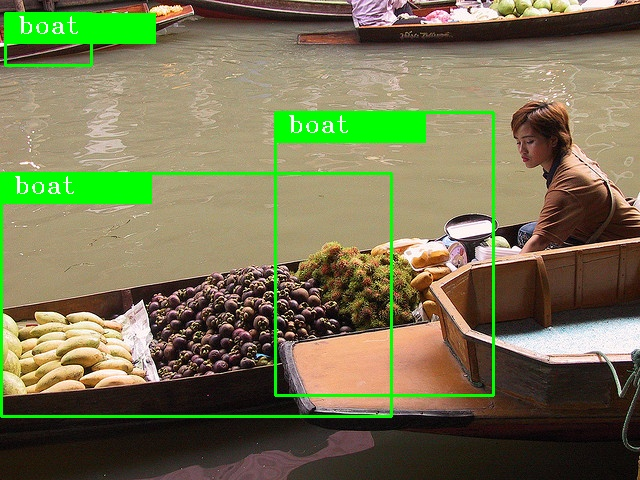
\includegraphics[width=1\textwidth]{ejemplo1.jpg}
	\end{subfigure}
	\begin{subfigure}{.48\textwidth}
		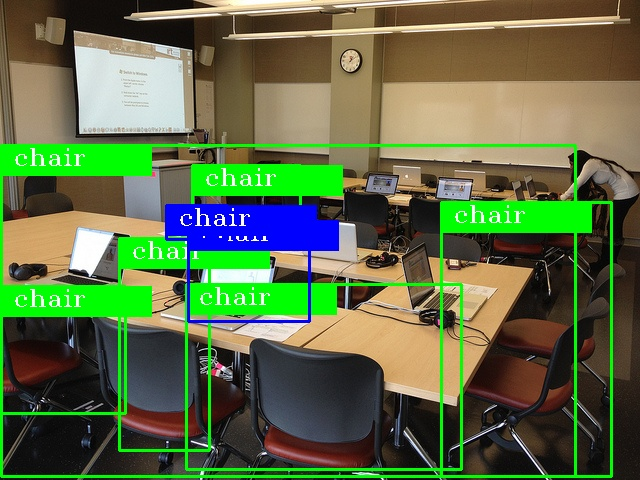
\includegraphics[width=1\textwidth]{ejemplo2.jpg}
	\end{subfigure}
	\begin{subfigure}{.45\textwidth}
		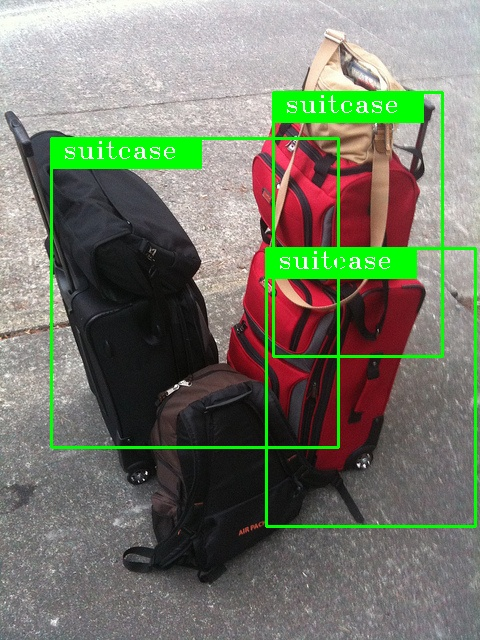
\includegraphics[width=1\textwidth]{ejemplo3.jpg}
	\end{subfigure}
	\begin{subfigure}{.45\textwidth}
		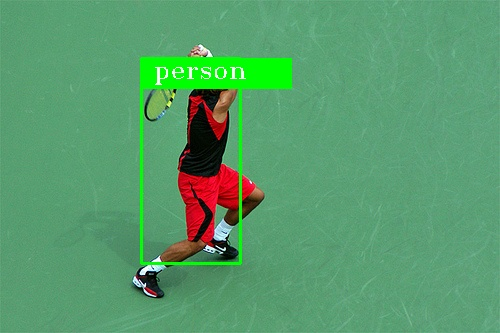
\includegraphics[width=1\textwidth]{ejemplo4.jpg}
		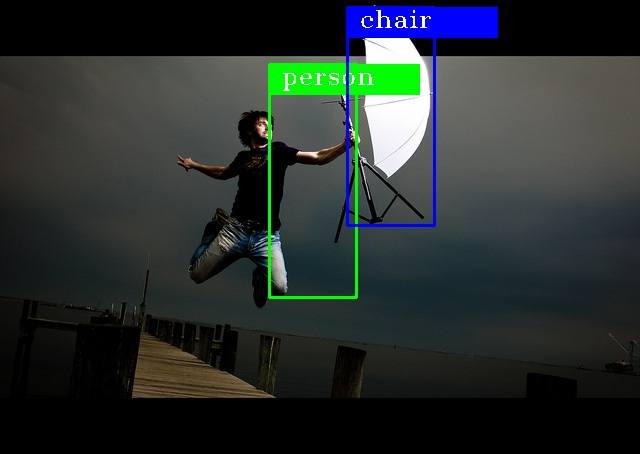
\includegraphics[width=1\textwidth]{ejemplo5.jpg}
	\end{subfigure}
	\caption{ejemplos}
	\label{fig:Ejmeplos}
\end{figure}
